\documentclass{beamer}
\usetheme{Antibes}
\usepackage{tikz}

% ---------- DISEÑO ------------------
\definecolor{verdeodi}{RGB}{53,113,105} %%%%%%%

\setbeamercolor*{structure}{bg=red,fg=verdeodi}

\setbeamercolor*{palette primary}{use=structure,fg=white,bg=structure.fg}
\setbeamercolor*{palette secondary}{use=structure,fg=white,bg=structure.fg!75}
\setbeamercolor*{palette tertiary}{use=structure,fg=white,bg=verdeodi}
\setbeamercolor*{palette quaternary}{fg=white,bg=verdeodi!50!black}

\setbeamercolor{section in toc}{fg=black,bg=white}
\setbeamercolor{alerted text}{use=structure,fg=structure.fg!50!verdeodi!80!black}

\setbeamercolor{titlelike}{parent=palette primary,fg=structure.fg!50!black}
\setbeamercolor{frametitle}{bg=verdeodi!50,fg=white}

\setbeamercolor*{titlelike}{parent=palette primary}
% ---------- O ------------------

\title{Estudio de la presencia de la aceleración de Fermi en billares rectangulares}
\subtitle{Trabajo fin de grado}
\author{Borja Sánchez González}
\institute{Universidad Nacional de Educación a Distancia}
\date{\empty}

\AtBeginSection[]
{
  \begin{frame}
    \frametitle{Table of Contents}
    \tableofcontents[currentsection]
  \end{frame}
}

\expandafter\def\expandafter\insertshorttitle\expandafter{%
  \insertshorttitle\hfill%
  \insertframenumber\,/\,\inserttotalframenumber}

\begin{document}
% -------- TITULO -----------
\begin{frame}
    \titlepage%
\end{frame}
% -------- O -----------

% -------- INDICE -----------
\begin{frame}
    \frametitle{Índice}
    \tableofcontents
\end{frame}
% -------- O -----------

% -------- INTRODUCCION-----------
\section{Introducción}

\subsection{¿Qué es la aceleración de Fermi?}

\begin{frame}
    \frametitle[prueb1]{Concepto}
    \begin{columns}
    \begin{column}{0.5\textwidth}
        \textbf{Aceleración de Fermi}\\
        Gran aumento de energía que adquiere una partícula tras varias interacciones.
    \end{column}

    \begin{column}{0.5\textwidth}
        \begin{figure}
            \includegraphics[scale=3]{images/aceleracion.pdf}    
        \end{figure}    
    \end{column}

    \end{columns}
\end{frame}

\begin{frame}
    \begin{columns}
        \begin{column}{0.5\textwidth}
            \begin{figure}
                \centering
                \includegraphics[scale=0.1]{images/Enrico_Fermi_1943-49.jpeg}  
                \caption{Enrico Fermi}  
            \end{figure}            
        \end{column}

        \begin{column}{0.5\textwidth}
            \begin{figure}
                \centering
                \includegraphics[scale=2.5]{images/Fermi-ulam.pdf}  
            \end{figure}            
        \end{column}
    \end{columns}
\end{frame}

\subsection{¿Qué es un billar?}

\begin{frame}
    \frametitle[prueb1]{Concepto}
    \begin{columns}
        \begin{column}{0.5\textwidth}
            \begin{figure}
                \includegraphics[scale=1]{images/bunimovich.pdf}    
                \caption{Bunimovich}
            \end{figure}  
            
        \end{column}
    
        \begin{column}{0.5\textwidth}
            \begin{figure}
                \includegraphics[scale=1]{images/sinai.pdf}
                \caption{Sinai}
            \end{figure}
        \end{column}
        \end{columns}
\end{frame}

\begin{frame}
    \frametitle[prueb1]{Concepto}
    \begin{align*}
        H = \dfrac{p^2}{2m} + V & & V = \begin{cases}
            0 \text{ en el interior de } \Omega \\
            \infty \text{ en el exterior de } \Omega
        \end{cases}
    \end{align*}
\end{frame}
% -------- O -----------

% -------- DINAMICA -----------
\section{Dinámica de la partícula}
\subsection{Ecuaciones de movimiento}


\begin{frame}
    \frametitle[prueb1]{Clásico}
    \begin{columns}
        \begin{column}{0.5\textwidth}
            \begin{figure}
                \centering
                \includegraphics[scale=1.2]{../images/elastic_collision.pdf}
            \end{figure}         
        \end{column}
        \begin{column}{0.5\textwidth}
            \centering
            Estacionario
            \begin{equation*}
                \mathbf{p}' = \mathbf{p} - 2\mathbf{n}(\mathbf{p} \cdot \mathbf{n})
            \end{equation*}\\
            \vspace{1cm}
            En movimiento
            \begin{equation*}
               \mathbf{u}' = \mathbf{u} - 2\mathbf{n}\left[(\mathbf{u} - \mathbf{w}) \cdot \mathbf{n}\right]
            \end{equation*}
        \end{column}
    \end{columns}
\end{frame}

\begin{frame}
    \frametitle[prueb1]{Relativista}
    \begin{columns}
        \begin{column}{0.5\textwidth}
            \begin{figure}
                \centering
                \includegraphics[scale=1]{../images/cambio_sistema_referencia.pdf}
            \end{figure}         
        \end{column}
        \hspace{1cm}
        \begin{column}{0.5\textwidth}
            \begin{figure}[H]
                \centering
                \includegraphics[scale=1.2]{../images/muro_vertical.pdf}
            \end{figure}
        \end{column}
    \end{columns}
\end{frame}

\begin{frame}[t]
    \frametitle[prueb1]{Relativista}
    \begin{columns}
        \begin{column}{0.5\textwidth}
            \begin{block}{Paso 1}
                \begin{align*}
                    r_{\parallel,S} &= \gamma\left( r_\parallel - w_\parallel t \right) \nonumber\\
                    r_{\perp, S} &= r_\perp  \\
                    t_S &= \gamma\left( t - \dfrac{r_\parallel w_\parallel}{c^2} \right) \nonumber
                \end{align*}
                \vspace{5.5mm}
            \end{block}
        \end{column}
        \begin{column}{0.5\textwidth}
        \end{column}
    \end{columns}
\end{frame}

\begin{frame}[t]
    \frametitle[prueb1]{Relativista}
    \begin{columns}
        \begin{column}{0.5\textwidth}
            \begin{block}{Paso 1}
                \begin{align*}
                    r_{\parallel,S} &= \gamma\left( r_\parallel - w_\parallel t \right) \nonumber\\
                    r_{\perp, S} &= r_\perp  \\
                    t_S &= \gamma\left( t - \dfrac{r_\parallel w_\parallel}{c^2} \right) \nonumber
                \end{align*}
                \vspace{5.5mm}
            \end{block}
        \end{column}
        \begin{column}{0.5\textwidth}
            \begin{block}{Paso 2}
                \begin{align*}
                    u_{\parallel,S} &= \dfrac{u_\parallel - w_\parallel}{1 - w_\parallel u_\parallel / c^2} \\[5mm]
                    u_{\perp,S} &= u_\perp\dfrac{\sqrt{1 - {(w_\parallel/c)}^2}}{1 - u_\parallel w_\parallel / c^2} 
                \end{align*}
            \end{block}
        \end{column}
    \end{columns}
    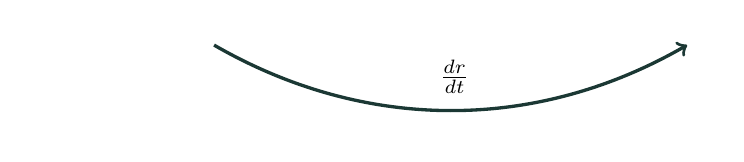
\begin{tikzpicture}[line/.style={->,shorten >=0.4cm,shorten <=0.4cm}, very thick]
        \draw[] (0,0) -- (0, 0);
        \path[verdeodi!50!black,bend right,line] (2,-0) edge (8.7,-0);
        \node at (5.4, -0.6) {$\frac{dr}{dt}$};
    \end{tikzpicture}
\end{frame}

\begin{frame}[t]
    \frametitle[prueb1]{Relativista}
    \begin{columns}
        \begin{column}{0.5\textwidth}
            \begin{block}{Paso 4}
                \begin{align*}
                    \bar{u}_{\parallel, S} &= -u_{\parallel, S} \\[9.5mm]
                    \bar{u}_{\perp, S} &= u_{\perp, S}
                \end{align*}
                \vspace{2.2mm}
            \end{block}
        \end{column}
        \begin{column}{0.5\textwidth}
        \end{column}
    \end{columns}
\end{frame}

\begin{frame}[t]
    \frametitle[prueb1]{Relativista}
    \begin{columns}
        \begin{column}{0.5\textwidth}
            \begin{block}{Paso 4}
                \begin{align*}
                    \bar{u}_{\parallel, S} &= -u_{\parallel, S} \\[9.5mm]
                    \bar{u}_{\perp, S} &= u_{\perp, S}
                \end{align*}
                \vspace{2.2mm}
            \end{block}
        \end{column}
        \begin{column}{0.5\textwidth}
            \begin{block}{Resultado}
                \begin{align*}
                    \bar{u}_\parallel &= \dfrac{-u_\parallel + 2w_\parallel - u_\parallel(w_\parallel/c)^2}{1 - 2w_\parallel u_\parallel / c^2 + (w_\parallel/c)^2} \\[5mm]
                    \bar{u}_\perp &= \dfrac{u_\perp\left(1 - (w_\parallel/c)^2\right)}{1 - 2w_\parallel u_\parallel / c^2 + (w_\parallel/c)^2}
                \end{align*}
            \end{block}
        \end{column}
    \end{columns}
\end{frame}

\begin{frame}
    \frametitle[prueb1]{Discretización}
    \begin{equation*}
        \left| u_n \right| = \left|  \dfrac{-u_{n-1} + 2w_n - u_{n-1}(w_n/c)^2}{1 - 2w_n u_{n-1}/c^2 + (w_n/c)^2} \right|
    \end{equation*}
\end{frame}

\begin{frame}
    \frametitle[prueb1]{Discretización}
    \begin{equation*}
        \left| u_n \right| = \left|  \dfrac{-u_{n-1} + 2w_n - u_{n-1}(w_n/c)^2}{1 - 2w_n u_{n-1}/c^2 + (w_n/c)^2} \right|
    \end{equation*}
    \begin{tikzpicture}[line/.style={->,shorten >=0.4cm,shorten <=0.4cm}, very thick]
        \draw[] (0,0) -- (0, 0);
        \draw[-stealth] (5.5, 0) -- (5.5, -2);
    \end{tikzpicture}
    \begin{equation*}
        u_n = -\dfrac{-u_{n-1} + 2w_n - u_{n-1}(w_n/c)^2}{1 - 2w_n u_{n-1}/c^2 + (w_n/c)^2}
    \end{equation*}
\end{frame}

\begin{frame}
    \frametitle[prueb1]{Cobwebs}{Clásico}
    \centering
    \begin{columns}
        \begin{column}{0.5\textwidth}
            \vspace{0.5cm}
            \begin{figure}
                \centering
                \includegraphics[scale=1]{../images/Cobweb_Classic_1D_A.pdf}
                \caption{$w_n>0$}
            \end{figure}  
        \end{column}
        \begin{column}{0.5\textwidth}
            \begin{figure}
                \centering
                \includegraphics[scale=1]{../images/Cobweb_Classic_1D_B.pdf}
                \caption{$w_n<0$}
            \end{figure}  
        \end{column}
    \end{columns}
\end{frame}

\begin{frame}
    \frametitle[prueb1]{Cobwebs}{Relativista}
    \centering
    \begin{columns}
        \begin{column}{0.5\textwidth}
            \vspace{0.cm}
            \begin{figure}
                \centering
                \includegraphics[scale=1]{../images/Cobweb_Relatitivy_1D_B.pdf}
                \caption{$w_n>0$}
            \end{figure}  
        \end{column}
        \begin{column}{0.5\textwidth}
            \begin{figure}
                \centering
                \includegraphics[scale=1]{../images/Cobweb_Relatitivy_1D_C.pdf}
                \caption{$w_n<0$}
            \end{figure}  
        \end{column}
    \end{columns}
\end{frame}

\begin{frame}
    \frametitle[prueb1]{Inelástico} 
\end{frame}

% -------- O -----------

% -------- SIMULACIONES -----------
\section{Simulaciones}
\subsection{Resultados numéricos}

\begin{frame}
    \frametitle[prueb1]{Clásico}
\end{frame}

\begin{frame}
    \frametitle[prueb1]{Relativista}
\end{frame}

\begin{frame}
    \frametitle[prueb1]{Inelástico}
\end{frame}
% -------- O -----------

% -------- CONCLUSIONES -----------
\section{Conclusiones}
% -------- O -----------

\begin{frame}
    \frametitle[prueb1]{Conclusiones}
\end{frame}


\end{document}

